\documentclass[titlepage,english,12pt]{article}
%%%%%%%%%%%%%%%%%%%%%%%%%%%%%%%%%%%%%%%%%%%%%%%%%%%%%%%%%%%%%%%%%%%%%%%%%%%%%%%%%%%%%%%%%%%%%%%%%%%%%%%%%%%%%%%%%%%%%%%%%%%%%%%%%%%%%%%%%%%%%%%%%%%%%%%%%%%%%%%%%%%%%%%%%%
\usepackage{amsmath,amsthm,amssymb}
\usepackage[margin=1in]{geometry}
\usepackage{authblk}
\usepackage{graphicx}
\usepackage{subfigure}
\usepackage{multirow}
\usepackage{array}
\usepackage{float}
\usepackage{natbib}

\pagestyle{plain}

% some definitions
\newtheorem{theorem}{Theorem}
\newtheorem{lemma}[theorem]{Lemma}

\newcommand{\E}{\mathop{\rm E}\nolimits} %expectation
\newcommand{\SE}{\mathop{\rm SE}\nolimits} %Standard Errors
\newcommand{\Var}{\mathop{\rm Var}\nolimits} %variance
\newcommand{\var}{\mathop{\rm var}\nolimits} %variance

\title{Smoothed quantile regression for residual lifetime in censored data}

\renewcommand\Affilfont{\normalfont\small}
\author{Kyu Hyun Kim}
\author{Sangwook Kang}
\affil{Department of Applied Statistics, Yonsei University}
\date{\today}

\begin{document}
	\maketitle
	
%%%%%%%%%%%%%%%%%%%%%%%%%%%% Abstract %%%%%%%%%%%%%%%%%%%%%%%%%%%%
\begin{abstract}
	
	We suggest a quantile regression method for residula lifetime given the prognostic factors and treatments at a ceratin followup time.
	To improve computational efficiency, we smooth an estimating function using induced smoothing approaches, 
	and use muliplier bootstrap and sandwich estimator method in finding a covariance matrix of regression estimator.
	We verify the performance of estimator in different combination of followup time point and censoring proportion of survival data in simulation settings,
	and apply proposed regression method to the longevity of dental restoration data from the Geriatric and Special Needs Dentistry Clinic at the University of Iowa Colloege of Dentistry (COD). 
	We also establish asymptotic normality and consistency of proposed estimator.\\
	
	\noindent{\it Keywords}: {Induced smoothing, Quantile regression, Residual lifetime regression, Sandwich estimator, Survival analysis}
	
\end{abstract}

%%%%%%%%%%%%%%%%%%%%%%%%%%%% Introduction %%%%%%%%%%%%%%%%%%%%%%%%%%%%
\section{Introduction}

	In general, most of medical researches are interested in how long patients will survive or how long effect of medicine or treatment lasts given a certain circumstances.
	The ultimate goal of both fields are estimate a remaining lifetime, and only difference is residual duration of what.
	For this reason, plenty of studies have focused on estimating mean survival time by various methods.
	However, regressions based on mean are not appropriate to estimate residual lifetime due to heterogeneity in survival data.
	To makeup this disadvantage of mean-based regression, past statisticians found an alternative ways, and most popular approach was quantile-based regression.
	
	
	First quantile regression model was introduced by \citet{koenker1978regression}, and lots of studies have been derived from this idea.
	\citet{jung2009regression} proposed a time-specific log-linear regression method that studies covariate effects on the conditional quantiles of residual lifetimes on a certain followup time point,
	and \citet{kim2012censored} suggested advanced regression applied inverse probability of censoring weighted (IPCW) estimator of \citet{van2003unified}, and an alternative way to estimte covariance matrix of the estimator or resamplingusing a simple empirical likelihood inference method.
	Those two apporaches find their estimators to solve own unsmoothed estimating equations using linear programming, however this approach is computationally inefficient. 
	Furthermore, it also caused the difficulty in variance estimation for censored quantile regression, thus some statisticians dealt with this problem applying alternative methods, such as \citet{kim2012censored}, or estimates approxmiated a covariance matrix, such as \cite{jung2009regression}. 
	However, they do not perfectly overcome disadvatage of unsmoothed estimating equation.
	
	 
	Fortunately, \citet{brown2007induced} introduced an induced smoothing method to solve unsmoothed issue.
	The induced smoothing idea smoothes unsmoothed estimating function by taking its expectation under the distribution of random perturbation.
	This concept makes solving estimating equation to computationally efficient, and also gives an opportunity to estimate variance.
	We suggest a variance estimation procedure derived from an approach of \citet{chiou2015semiparametric} based on multiplier boothstrapping and sandwich estimator.
	Because a sandwich estimator method is developed to estimate variance with computational efficiency, if an estimator satisfies asymptotic properties and consistency, it is very useful to estimate variance.
	
	The rest of the article is organized as follows.
	In section 2, we introduce the process how to approach smoothed quantile regression estimator for residual lifetime. 
	We discuss simulation results in section 3, and real data analysis in section 4.
	Discussion and some necessary proofs are at the end of this article.\\
	
%%%%%%%%%%%%%%%%%%%%%%%%%%%% Body %%%%%%%%%%%%%%%%%%%%%%%%%%%%	
\section{Censored quantile regression for residual lifetime with induced smoothing}

%%%%%%%%%%%%%%%%%%%%%%%%%%%% No censoring assumption %%%%%%%%%%%%%%%%%%%%%%%%%%%%
\subsection{AFT model with no censored data}

	We start from scenario where random sample subject to no censoring: $\{T_i, X_i\}_{i=1}^{n}$, where $T_i, X_i$ denote the failure time, and covariate values of $i^{th}$ subject respectively.\\
		
	\noindent $\theta_{\tau}(t_0)$ is $\tau$-th quantile of residual lifetime at followup time $t_0$, and we simply express it as $\theta_{\tau}$. Corresponding to the AFT model and regression quantiles of residual lifetime, the $\tau$-th quantile of residual lifetime given the covariate $X_i$ is given by
	\begin{equation} \label{eq:1}
	\theta_{\tau}=log(T_i-t_0)=X_{i}^{\prime}\beta(\tau, t_0)+\epsilon_i
	\end{equation}
	where $\beta(\tau, t_0)$ represents $\tau$-th quantile regression coefficient given covariate $X_i$ and followup time $t_0$, and we simply use $\beta$ instead of $\beta(\tau, t_0)$. $\epsilon_i$ is independent and have zero $\tau$-th quantile.\\
	
	\noindent In this case, the $\tau$-th quantile residual lifetime quantile is solution of estimating equation:
	\begin{equation} \label{eq:2}
	0 = n^{-1}\sum_{i=1}^{n}I[(T_i-t_0)\leq\theta_{\tau}]-(1-\tau)I[T_i \leq t_0]-\tau
	\end{equation}

	\noindent After some manipulations, estimating equation for $\tau$-th quantile regression coefficient $\beta$ is
	\begin{equation} \label{eq:3}
	0 = n^{-1}\sum_{i=0}^{n}I[T_i \ge t_0] X_i I \Big(I\{\log(T_i - t_0) \leq X_i^{\prime}\beta\} - \tau \Big)
	\end{equation}

%%%%%%%%%%%%%%%%%%%%%%%%%%%% Censoring assumption %%%%%%%%%%%%%%%%%%%%%%%%%%%%
\subsection{AFT model with censored data}

	\noindent And we consider concept of censoring of subject. Suppose n iid $\{T_i, X_i\}_{i=1}^{n}$ are generated from model (\ref{eq:1}), and we have right censored data $\{Z_i, \delta_i, X_i \}_{i=1}^{n}$ where $Z_i=min(T_i,C_i), \delta_i = I[T_i \leq C_i]$ are independent. In this case, we need to consider weight $w_i$, which are the probability that Kaplan-Meier estimator based on $\{Z_i, \delta_i \}_{i=1}^{n}$ assigns on the case $(Z_i, \delta_i)$. For this weight, we use inverse probability of censoring weighting (IPCW) technique \citet{robins1992recovery}.\\
	
	\noindent Therefore, estimating equation of censored regression residual quantile estimator is:
	\begin{equation} \label{eq:4}
	U_n(\beta) = 0 = n^{-1}\sum_{i=1}^{n}I[Z_i \ge t_0] X_i \Big(I\{\log(Z_i - t_0) \leq X_i^{\prime}\beta\} \frac{\delta_i}{\hat{G}(Z_i)}  -\tau \Big)
	\end{equation}
	where $\hat{G}(Z_i)$ is the Kaplan-Meier estimate of the survival unction of the censoring variable $C_i$. We prove consistancy and asymptotic properties of unsmoothed estimator in appendix.\\
	\\
	There is similar estimating equation of censored regression residual quantile estimator that suggested at \citet{pang2012variance} and \citet{kim2012censored}. Both estimating equations used IPCW as weight to apply censored data, however, only difference is the position of weight. Both equations are theoretically correct equations, and \citet{peng2009competing} also similar estimating equation.\\

%%%%%%%%%%%%%%%%%%%%%%%%%%%% Induced smoothing %%%%%%%%%%%%%%%%%%%%%%%%%%%%
\subsection{Induced smoothing approach}

	\noindent Even though solving equation (\ref{eq:4}) is possible by using linear programming approach, it has much intensive computation issue. To minimize computation burden, we apply induced smoothing method, proposed by \citet{brown2007induced}. By the asymptotic normality of $\hat{\beta}$, we can express $\hat{\beta} = \beta+\textbf{H}^{1/2}V$, where $H = n^{-1}\Gamma,\ V \sim N(0, I_p)$, and $I_p$ is the $p \times p $ identity matrix. After applying induced smoothing approach to equation (\ref{eq:4})
	
	\begin{equation} \label{eq:5}
	\tilde{U}_n(\beta, \textbf{H}) = E_v \{U_n(\beta+\textbf{H}^{1/2}V)\} = n^{-1} \sum_{i=1}^{n} I[Z_i \geq t_0] X_i \Big\{\tau - \frac{\delta_i}{\hat{G}(Z_i)}\Phi\Big(\frac{X_i^\prime\beta-log(Z_i-t_0)}{\sqrt{X_i^{\prime} \textbf{H} X_{i}}}\Big)\Big\}
	\end{equation} 
	where $\Phi(\cdot)$ is the standard normal cumulative distribution function. As \citet{pang2012variance} proposed, we use a positive definite $p \times p$ matrix $\tilde{\textbf{H}} = O(n^{-1})$ as a smoothing matrix $\textbf{H}$.\\ Estimated $\beta$ from equation \ref{eq:5} is also consistent and asymptotically normal by \ref{thm:1} under below regularity conditions C1-C3:
	\begin{enumerate}
		\item[C1] The conditional error distribution functions, $F_{i}(\cdot\mid X_{i})^{n}_{i=1}$, are absolutely continuous with continuous densities $f_{i}(\cdot\mid X_{i})$ uniformly bounded away from $0$ and $\infty$ in a neighborhood of $0$, and $f_{i}^{\prime}(\cdot\mid X_{i})$ exists and is uniformly bounded on the real line.
		\item[C2] For each $i=1,\dots, n, X_{i}$ satisfies the following conditions:
		\begin{flushleft}
			(a) $n^{-1}\Sigma_{i=1}^{n} X_{i} X_{i}^{\prime}f_{i}(0\mid X_{i})$ converges to a positive definite matrix \textbf{A};\\
			(b) sup$_{i}\lVert X_{i} \rVert < \infty\ $, where $\lVert \cdot \rVert$ denotes the Euclidean norm.\\
		\end{flushleft}
		\item[C3] There exists $L>0$ such that $P(C>L)=0$ and $P(C=L)\geq\nu$, where $\nu$ is some positive constant.
	\end{enumerate} 

	\begin{theorem} \label{thm:1}
	Assume condition $1-3$ hold, and the smoothing matrix $H$ is positive definite and $O(n^{-1})$, as $n\to\infty$ then we have
		\begin{center}
			$n^{1/2}(\hat{\beta}_{IS}-\beta_0) \xrightarrow{d} \mathcal{N}(0,\Gamma)$
		\end{center}
	\end{theorem}
	
	\noindent We prove above theorem \ref{thm:1} in appendix.\\
	
	\noindent To estimate the asymptotic variance of $\hat{\beta}_{IS}$, we use sandwich estimators, which is computationally more efficient than full-multiplier bootstrap approach based on \citet{chiou2015semiparametric}. 
	
	\noindent For sandwich estimator, $\Sigma(\beta_0)$, two estimators, $A(\beta_0)$ and $V(\beta_0)$, are necessary. For estimating $A(\beta_0)$, 
	we evaluate $A_n(\beta_0)$, the derivative of the smoothed estimating function:
	
	\begin{equation} \label{eq:6}
	A_n(\beta_0) = \frac{\partial \tilde{U}_n(\hat{\beta}_{IS}, \tilde{\textbf{H}})}{\partial \beta} = n^{-1}\sum_{i=1}^{n} I[Z_i>t_0] X_i \frac{\delta_i}{\hat{G}(Z_i)} \phi\bigg(\frac{{X_i}^{\prime}\hat{\beta}_{IS}-\log(Z_i-t_0)}{\sqrt{{X_i}^{\prime}\tilde{\textbf{H}} X_i}}\bigg)\bigg(\frac{-{X_i}}{\sqrt{{X_i}^{\prime} \tilde{\textbf{H}} {X_i}}}\bigg)
	\end{equation}
	
	\noindent at $\hat{\beta}_{IS}$, which is the solution of estimating equation (\ref{eq:5}), where $\phi \{ \cdot \}$ is the density function of a standard normal distribution.\\
	
	\noindent For estimating $V(\beta_0)$, we generate iid positive multiplier $\eta_i, i=1,...,n,$ that are independent of the observed data from $\exp(1)$, and make perturbed estimating equation, $\tilde{U}^{\star}_n(\beta, \textbf{H})$, with generated $\eta_i$:
	
	\begin{equation} \label{eq:7}
	\tilde{U}^{\star}_n(\beta, \tilde{\textbf{H}}) = n^{-1} \sum_{i=1}^{n} I[Z_i \geq t_0] X_i \eta_i \Big\{\tau - \frac{\delta_i}{\hat{G}(Z_i)}\Phi\Big(\frac{X_i^\prime\beta-log(Z_i-t_0)}{\sqrt{X_i^{\prime} \tilde{\textbf{H}} X_{i}}}\Big)\Big\}
	\end{equation}
	
	\noindent We evaluate $\tilde{U}^{\star}_n(\beta, \tilde{\textbf{H}})$ at $\hat{\beta}_{IS}$. Repeating same process $m$ times with new multipliers, and find sample variance of $\{\tilde{U}^{\star (1)}_n(\beta, \tilde{\textbf{H}}),..., \tilde{U}^{\star (m)}_n(\beta, \tilde{\textbf{H}})\}$. $V(\beta_0)$ is approxiamated to sample variance of $\tilde{U}^{\star}_n(\beta, \tilde{\textbf{H}})$.
	
	\noindent Using above $A(\beta_0)$, and $V(\beta_0)$, $\Sigma(\beta_0)$ is:
	\begin{equation} \label{eq:8}
	\Sigma(\beta_0) = A(\beta_0)^T V(\beta_0) A(\beta_0)
	\end{equation}
	
%%%%%%%%%%%%%%%%%%%%%%%%%%%% Simulation %%%%%%%%%%%%%%%%%%%%%%%%%%%%
\section{Simulation}

	To verify performance of smoothed estimator, we used same simple regression simulation setting that provided by \citet{jung2009regression}. Covariate $X_i$ is a binary covariate, 0 for control and 1 for treatment group. $Z_i = min(T_i, C_i)$ where $T_i$ generated from Weibull regression model with one binary covariate $X_i$ and intercept and where $C_i$ generated from uniform distribution with range 0 and c, which is adjusted for censoring proportion. One dataset size was 200, and 2000 simulations were performed for every combination of $t_0$ and censoring proportion. In variance estimating process, we need to fix how many $\tilde{U}^{\star }_n(\beta, \tilde{\textbf{H}})$ we will use to find sample variance. Comparing sample variance of 100 $V(\beta_0)$s and sample variance of 500 $V(\beta_0)$s, we conclude that 100 $\tilde{U}^{\star }_n(\beta, \tilde{\textbf{H}})$s are close enough to $V(\beta_0)$.
	
	From table \ref{table:1} to table \ref{table:3}, we verify the performance of suggested estimator when covariate does not affect residual lifetime, which means $\beta_{t_0}^{(1)} = 0$. Based on \citet{jung2009regression} simulation setting, true parameter $\beta_{t_0}^{(0)} = 1.61, 1.41, 1.22, 1.04$ at $t_0 = 0, 1, 2, 3$. $\beta^(0)$ and $\beta^(1)$ are mean of empirical estimates of true paramters $\beta^(0), \beta^(1)$, and SE is mean of standard error of empirical estimates of each true parameter. SD is standard deviation of empirical estimates, and Coverage is proportion that true parameter are included in $95\%$ confidence interval of proposed estimates. 

%%%%%%%%%%%%%%%%%%%%%%%%%%%% beta_1 =0 setting with at 3 difference quantile %%%%%%%%%%%%%%%%%%%%%%%%%%%%

	\begin{table}[H] \label{table:1}
		\caption{Estimates of $25\%$ quantile residual lifetime when $\beta^{(1)}=0$}
		\centering
		\begin{tabular}{|c|c|c|c|c|c|c|c|c|c|}
			\hline
			\multirow{2}{*}{$t_0$} & \multirow{2}{*}{censor} & \multicolumn{4}{c|}{$\beta^{(0)}$} & \multicolumn{4}{c|}{$\beta^{(1)}$}\\ \cline{3-10}
			& & $\beta^{(0)}$ & SE & SD  & Coverage  & $\beta^{(1)}$ & SE & SD & Coverage\\
			\hline\hline
			\multirow{4}{*}{$t_0=0$} & 0\% & 1.607 & 0.069 & 0.069 & 0.931 & 0.000 & 0.098 & 0.069 & 0.946 \\
			& 10\% & 1.608 & 0.073 & 0.069 & 0.937 & 0.000 & 0.104 & 0.069 & 0.944 \\
			& 30\% & 1.608 & 0.083 & 0.081 & 0.926 & 0.001 & 0.119 & 0.081 & 0.941 \\
			& 50\% & 1.606 & 0.096 & 0.091 & 0.924 & 0.003 & 0.137 & 0.091 & 0.933 \\
			\hline
			\multirow{4}{*}{$t_0=1$} & 0\% & 1.406 & 0.084 & 0.084 & 0.927 & -0.001 & 0.120 & 0.084 & 0.940 \\
			& 10\% & 1.408 & 0.089 & 0.090 & 0.916 & -0.003 & 0.127 & 0.090 & 0.934 \\
			& 30\% & 1.403& 0.103 & 0.098 & 0.928 & 0.002 & 0.147 & 0.098 & 0.932 \\
			& 50\% & 1.408 & 0.120 & 0.115 & 0.908 & -0.001 & 0.174 & 0.115 & 0.938 \\
			\hline
			\multirow{4}{*}{$t_0=2$} & 0\% & 1.214 & 0.100 & 0.099 & 0.924 & 0.002 & 0.143 & 0.099 & 0.943 \\
			& 10\% & 1.214 & 0.108 & 0.106 & 0.918 & 0.000 & 0.154 & 0.106 & 0.942 \\
			& 30\% & 1.215 & 0.126 & 0.121 & 0.923 & -0.002 & 0.181 & 0.121 & 0.938 \\
			& 50\% & 1.220 & 0.151 & 0.144 & 0.912 & 0.000 & 0.222 & 0.144 & 0.925 \\
			\hline
			\multirow{4}{*}{$t_0=3$} & 0\% & 1.038 & 0.120 & 0.121 & 0.913 & -0.004 & 0.171 & 0.121 & 0.923 \\
			& 10\% & 1.038 & 0.129 & 0.133 & 0.904 & -0.004 & 0.186 & 0.133 & 0.934 \\
			& 30\% & 1.037 & 0.157 & 0.153 & 0.914 & 0.005 & 0.225 & 0.153 & 0.935 \\
			& 50\% & 1.040 & 0.186 & 0.177 & 0.906 & 0.005 & 0.284 & 0.177 & 0.937 \\
			\hline
		\end{tabular}
	\end{table}

	\begin{table}[H] \label{table:2}
		\caption{Estimates of $50\%$ quantile residual lifetime when $\beta^{(1)}=0$}
		\centering
		\begin{tabular}{|c|c|c|c|c|c|c|c|c|c|}
			\hline
			\multirow{2}{*}{$t_0$} & \multirow{2}{*}{censor} & \multicolumn{4}{c|}{$\beta^{(0)}$} & \multicolumn{4}{c|}{$\beta^{(1)}$}\\ \cline{3-10}
			& & $\beta^{(0)}$ & SE & SD  & Coverage  & $\beta^{(1)}$ & SE & SD & Coverage\\
			\hline\hline
			\multirow{4}{*}{$t_0=0$} & 0\% & 1.607 & 0.069 & 0.069 & 0.931 & 0.000 & 0.098 & 0.069 & 0.946 \\
			& 10\% & 1.607 & 0.073 & 0.069 & 0.937 & -0.001 & 0.104 & 0.069 & 0.944 \\
			& 30\% & 1.608 & 0.083 & 0.081 & 0.926 & -0.002 & 0.119 & 0.081 & 0.941 \\
			& 50\% & 1.606 & 0.096 & 0.091 & 0.924 & 0.003 & 0.137 & 0.091 & 0.933 \\
			\hline
			\multirow{4}{*}{$t_0=1$} & 0\% & 1.406 & 0.084 & 0.084 & 0.927 & -0.001 & 0.120 & 0.084 & 0.940 \\
			& 10\% & 1.408 & 0.090 & 0.090 & 0.916 & -0.003 & 0.127 & 0.090 & 0.934 \\
			& 30\% & 1.403 & 0.103 & 0.098 & 0.928 & 0.002 & 0.147 & 0.098 & 0.932 \\
			& 50\% & 1.408 & 0.120 & 0.115 & 0.908 & -0.001 & 0.174 & 0.115 & 0.938 \\
			\hline
			\multirow{4}{*}{$t_0=2$} & 0\% & 1.214 & 0.100 & 0.099 & 0.924 & 0.002 & 0.143 & 0.099 & 0.943 \\
			& 10\% & 1.214 & 0.108 & 0.106 & 0.918 & 0.000 & 0.154 & 0.106 & 0.942 \\
			& 30\% & 1.215 & 0.126 & 0.121 & 0.922 & -0.002 & 0.181 & 0.121 & 0.938 \\
			& 50\% & 1.220 & 0.151 & 0.144 & 0.911 & 0.000 & 0.222 & 0.144 & 0.925 \\
			\hline
			\multirow{4}{*}{$t_0=3$} & 0\% & 1.038 & 0.120 & 0.121 & 0.913 & -0.004 & 0.171 & 0.121 & 0.923 \\
			& 10\% & 1.038 & 0.129 & 0.133 & 0.904 & -0.003 & 0.186 & 0.133 & 0.934 \\
			& 30\% & 1.036 & 0.157 & 0.153 & 0.914 & 0.005 & 0.225 & 0.153 & 0.935 \\
			& 50\% & 1.040 & 0.186 & 0.177 & 0.906 & 0.005 & 0.284 & 0.177 & 0.937 \\
			\hline
		\end{tabular}
	\end{table}
			
	\begin{table}[H] \label{table:3}
		\caption{Estimates of $75\%$ quantile residual lifetime when $\beta^{(1)}=0$}
		\centering
		\begin{tabular}{|c|c|c|c|c|c|c|c|c|c|}
			\hline
			\multirow{2}{*}{$t_0$} & \multirow{2}{*}{censor} & \multicolumn{4}{c|}{$\beta^{(0)}$} & \multicolumn{4}{c|}{$\beta^{(1)}$}\\ \cline{3-10}
			& & $\beta^{(0)}$ & SE & SD  & Coverage  & $\beta^{(1)}$ & SE & SD & Coverage\\
			\hline\hline
			\multirow{4}{*}{$t_0=0$} & 0\% & 1.609 & 0.058 & 0.058 & 0.926 & 0.003 & 0.082 & 0.058 & 0.938 \\
			& 10\% & 1.610 & 0.069 & 0.066 & 0.951 & 0.001 & 0.098 & 0.066 & 0.941 \\
			& 30\% & 1.610 & 0.092 & 0.080 & 0.955 & 0.008 & 0.133 & 0.080 & 0.948 \\
			& 50\% & 1.615 & 0.133 & 0.101 & 0.948 & 0.002 & 0.200 & 0.101 & 0.961 \\
			\hline
			\multirow{4}{*}{$t_0=1$} & 0\% & 1.410 & 0.072 & 0.075 & 0.917 & -0.001 & 0.103 & 0.075 & 0.931 \\
			& 10\% & 1.410 & 0.086 & 0.081 & 0.936 & 0.002 & 0.122 & 0.081 & 0.942 \\
			& 30\% & 1.410 & 0.117 & 0.104 & 0.940 & 0.010 & 0.171 & 0.104 & 0.948 \\
			& 50\% & 1.396 & 0.207 & 0.120 & 0.944 & 0.014 & 0.327 & 0.120 & 0.969 \\
			\hline
			\multirow{4}{*}{$t_0=2$} & 0\% & 1.215 & 0.090 & 0.092 & 0.906 & 0.005 & 0.129 & 0.092 & 0.930 \\
			& 10\% & 1.219 & 0.109 & 0.103 & 0.935 & 0.000 & 0.156 & 0.103 & 0.934 \\
			& 30\% & 1.222 & 0.154 & 0.140 & 0.926 & 0.006 & 0.228 & 0.140 & 0.929 \\
			& 50\% & 1.175 & 0.264 & 0.136 & 0.941 & 0.018 & 0.530 & 0.136 & 0.987 \\
			\hline
			\multirow{4}{*}{$t_0=3$} & 0\% & 1.036 & 0.116 & 0.121 & 0.905 & 0.000 & 0.166 & 0.121 & 0.929 \\
			& 10\% & 1.037 & 0.140 & 0.138 & 0.907 & 0.006 & 0.205 & 0.138 & 0.925 \\
			& 30\% & 1.040 & 0.215 & 0.191 & 0.904 & 0.016 & 0.330 & 0.191 & 0.945 \\
			& 50\% & 0.946 & 0.651 & 0.177 & 0.937 & 0.036 & 0.905 & 0.177 & 0.991 \\	
			\hline
		\end{tabular}
	\end{table}

	In every combination of $t_0$, censoring proportion, and estimated quantile, proposed estimator is quite close to true paramter except for estimating high qunatile $75\%$ from data with high censoring proportion, $70\%$. Furthermore, small data size due to large $t_0$ makes estimating true parameter more difficult.\\
	
	From table \ref{table:4} to table \ref{table:6}, we verify that smoothed estimator is able to estimate an effect of covariate. In this simulation scenario, we add one more assumption that the difference in residual time between two groups are 5. Then, true parameter $\beta_{t_0}^{(0)} = 1.61, 1.41, 1.22, 1.04$ at $t_0 = 0, 1, 2, 3$ and $\beta_{t_0}^{(1)} = 0.69, 0.80, 0.91, 1.02$ at $t_0 = 0, 1, 2, 3$.

%%%%%%%%%%%%%%%%%%%%%%%%%%%% beta_1 \neq 0 setting with at 3 difference quantile %%%%%%%%%%%%%%%%%%%%%%%%%%%%

	\begin{table}[H] \label{table:4}
		\caption{Estimates of $25\%$ quantile residual lifetime when $\beta^{(1)} \neq 0$}
		\centering
		\begin{tabular}{|c|c|c|c|c|c|c|c|c|c|}
			\hline
			\multirow{2}{*}{$t_0$} & \multirow{2}{*}{censor} & \multicolumn{4}{c|}{$\beta^{(0)}$} & \multicolumn{4}{c|}{$\beta^{(1)}$}\\ \cline{3-10}
			& & $\beta^{(0)}$ & SE & SD  & Coverage  & $\beta^{(1)}$ & SE & SD & Coverage\\
			\hline\hline
			\multirow{4}{*}{$t_0=0$} & 0\% & 1.604 & 0.096 & 0.098 & 0.910 & 0.692 & 0.137 & 0.098 & 0.929 \\
			& 10\% & 1.604 & 0.098 & 0.099 & 0.908 & 0.693 & 0.141 & 0.099 & 0.934 \\
			& 30\% & 1.605 & 0.102 & 0.102 & 0.904 & 0.693 & 0.150 & 0.102 & 0.933 \\
			& 50\% & 1.606 & 0.106 & 0.107 & 0.905 & 0.692 & 0.162 & 0.107 & 0.937 \\
			\hline
			\multirow{4}{*}{$t_0=1$} & 0\% & 1.403 & 0.116 & 0.116 & 0.909 & 0.789 & 0.159 & 0.116 & 0.933 \\
			& 10\% & 1.410 & 0.119 & 0.119 & 0.907 & 0.787 & 0.164 & 0.119 & 0.937 \\
			& 30\% & 1.399 & 0.124 & 0.124 & 0.898 & 0.797 & 0.176 & 0.124 & 0.925 \\
			& 50\% & 1.407 & 0.129 & 0.128 & 0.905 & 0.793 & 0.188 & 0.128 & 0.930 \\
			\hline
			\multirow{4}{*}{$t_0=2$} & 0\% & 1.210 & 0.137 & 0.140 & 0.894 & 0.884 & 0.182 & 0.140 & 0.923 \\
			& 10\% & 1.209 & 0.142 & 0.140 & 0.908 & 0.886 & 0.191 & 0.140 & 0.927 \\
			& 30\% & 1.216 & 0.144 & 0.146 & 0.900 & 0.878 & 0.201 & 0.146 & 0.927 \\
			& 50\% & 1.209 & 0.152 & 0.152 & 0.899 & 0.893 & 0.218 & 0.152 & 0.925 \\
			\hline
			\multirow{4}{*}{$t_0=3$} & 0\% & 1.031 & 0.154 & 0.154 & 0.895 & 0.965 & 0.204 & 0.154 & 0.917 \\
			& 10\% & 1.032 & 0.158 & 0.162 & 0.886 & 0.972 & 0.211 & 0.162 & 0.923 \\
			& 30\% & 1.040 & 0.166 & 0.168 & 0.889 & 0.957 & 0.226 & 0.168 & 0.909 \\
			& 50\% & 1.037 & 0.182 & 0.174 & 0.891 & 0.963 & 0.254 & 0.174 & 0.909 \\
			\hline
		\end{tabular}
	\end{table}
	
	\begin{table}[H] \label{table:5}
		\caption{Estimates of $50\%$ quantile residual lifetime when $\beta^{(1)} \neq 0$}
		\centering
		\begin{tabular}{|c|c|c|c|c|c|c|c|c|c|}
			\hline
			\multirow{2}{*}{$t_0$} & \multirow{2}{*}{censor} & \multicolumn{4}{c|}{$\beta^{(0)}$} & \multicolumn{4}{c|}{$\beta^{(1)}$}\\ \cline{3-10}
			& & $\beta^{(0)}$ & SE & SD  & Coverage  & $\beta^{(1)}$ & SE & SD & Coverage\\
			\hline\hline
			\multirow{4}{*}{$t_0=0$} & 0\% & 1.607 & 0.068 & 0.068 & 0.921 & 0.692 & 0.097 & 0.068 & 0.949 \\
			& 10\% & 1.607 & 0.072 & 0.070 & 0.931 & 0.691 & 0.104 & 0.070 & 0.944 \\
			& 30\% & 1.606 & 0.078 & 0.075 & 0.932 & 0.695 & 0.119 & 0.075 & 0.943 \\
			& 50\% & 1.606 & 0.086 & 0.081 & 0.933 & 0.695 & 0.149 & 0.081 & 0.945 \\
			\hline
			\multirow{4}{*}{$t_0=1$} & 0\% & 1.408 & 0.084 & 0.086 & 0.912 & 0.790 & 0.114 & 0.086 & 0.932 \\
			& 10\% & 1.406 & 0.087 & 0.088 & 0.930 & 0.790 & 0.121 & 0.088 & 0.944 \\
			& 30\% & 1.408 & 0.095 & 0.095 & 0.922 & 0.791 & 0.139 & 0.095 & 0.938 \\
			& 50\% & 1.409 & 0.105 & 0.103 & 0.925 & 0.789 & 0.190 & 0.103 & 0.943 \\
			\hline
			\multirow{4}{*}{$t_0=2$} & 0\% & 1.216 & 0.100 & 0.100 & 0.918 & 0.884 & 0.132 & 0.100 & 0.937 \\
			& 10\% & 1.217 & 0.106 & 0.103 & 0.922 & 0.880 & 0.142 & 0.103 & 0.946 \\
			& 30\% & 1.215 & 0.116 & 0.114 & 0.916 & 0.879 & 0.164 & 0.114 & 0.931 \\
			& 50\% & 1.216 & 0.131 & 0.123 & 0.915 & 0.872 & 0.239 & 0.123 & 0.941 \\
			\hline
			\multirow{4}{*}{$t_0=3$} & 0\% & 1.030 & 0.121 & 0.122 & 0.915 & 0.972 & 0.154 & 0.122 & 0.913 \\
			& 10\% & 1.037 & 0.125 & 0.127 & 0.896 & 0.965 & 0.163 & 0.127 & 0.902 \\
			& 30\% & 1.037 & 0.137 & 0.137 & 0.902 & 0.964 & 0.187 & 0.137 & 0.927 \\
			& 50\% & 1.037 & 0.158 & 0.154 & 0.904 & 0.943 & 0.312 & 0.154 & 0.925 \\
			\hline
		\end{tabular}
	\end{table}

	\begin{table}[H] \label{table:6}
		\caption{Estimates of $75\%$ quantile residual lifetime when $\beta^{(1)} \neq 0$}
		\centering
		\begin{tabular}{|c|c|c|c|c|c|c|c|c|c|}
			\hline
			\multirow{2}{*}{$t_0$} & \multirow{2}{*}{censor} & \multicolumn{4}{c|}{$\beta^{(0)}$} & \multicolumn{4}{c|}{$\beta^{(1)}$}\\ \cline{3-10}
			& & $\beta^{(0)}$ & SE & SD  & Coverage  & $\beta^{(1)}$ & SE & SD & Coverage\\
			\hline\hline
			\multirow{4}{*}{$t_0=0$} & 0\% & 1.610 & 0.058 & 0.0593 & 0.922 & 0.695 & 0.082 & 0.059 & 0.944 \\
			& 10\% & 1.610 & 0.066 & 0.063 & 0.938 & 0.695 & 0.098 & 0.063 & 0.940 \\
			& 30\% & 1.611 & 0.080 & 0.074 & 0.939 & 0.698 & 0.134 & 0.074 & 0.955 \\
			& 50\% & 1.627 & 0.105 & 0.093 & 0.961 & 0.614 & 0.430 & 0.093 & 0.955 \\
			\hline
			\multirow{4}{*}{$t_0=1$} & 0\% & 1.408 & 0.072 & 0.073 & 0.929 & 0.795 & 0.098 & 0.073 & 0.935 \\
			& 10\% & 1.407 & 0.081 & 0.079 & 0.933 & 0.796 & 0.115 & 0.079 & 0.947 \\
			& 30\% & 1.410 & 0.097 & 0.092 & 0.935 & 0.799 & 0.159 & 0.092 & 0.951 \\
			& 50\% & 1.435 & 0.132 & 0.118 & 0.935 & 0.654 & 0.618 & 0.118 & 0.923 \\
			\hline
			\multirow{4}{*}{$t_0=2$} & 0\% & 1.215 & 0.091 & 0.092 & 0.9212 & 0.889 & 0.117 & 0.092 & 0.927 \\
			& 10\% & 1.218 & 0.101 & 0.101 & 0.912 & 0.888 & 0.138 & 0.101 & 0.934 \\
			& 30\% & 1.221 & 0.125 & 0.119 & 0.917 & 0.887 & 0.200 & 0.119 & 0.946 \\
			& 50\% & 1.251 & 0.175 & 0.150 & 0.931 & 0.689 & 0.858 & 0.150 & 0.881 \\
			\hline
			\multirow{4}{*}{$t_0=3$} & 0\% & 1.033 & 0.117 & 0.115 & 0.919 & 0.974 & 0.144 & 0.115 & 0.916 \\
			& 10\% & 1.037 & 0.130 & 0.126 & 0.907 & 0.968 & 0.169 & 0.126 & 0.922 \\
			& 30\% & 1.046 & 0.158 & 0.150 & 0.919 & 0.970 & 0.241 & 0.150 & 0.943 \\
			& 50\% & 1.079 & 0.240 & 0.209 & 0.906 & 0.741 & 0.604 & 0.209 & 0.893 \\	
			\hline
		\end{tabular}
	\end{table}

	In data with high censoring proportion, estimating $\beta$ is unstable. When we find a solution for proposed estimating equation (\ref{eq:5}), we use nleqslv function in nleqslv R package. However, solutions from high censored proportion data are not unique or unsolvable, other nonlinear equation solvers also have similar issues. If both estimating quantile and censored proportion are high, we are hard to find solution. Futhermore, size of dataset affects performance of proposed estimator. Smaller dataset caused more error in solving the estimating equation, and also shows poor performance. 

%%%%%%%%%%%%%%%%%%%%%%%%%%%% High censoring proporation cases table %%%%%%%%%%%%%%%%%%%%%%%%%%%%
	
	\begin{table}[H] \label{table:7}
		\caption{Various quantile estimates of residual lifetime with high censoring ($70\%$) when $\beta^{(1)} = 0$. When estimating quantile is high, results show big differences with true beta, or cannot estimate.}
		\centering
		\begin{tabular}{|c|c|c|c|c|c|c|c|c|c|}
			\hline
			\multirow{2}{*}{$t_0$} & \multirow{2}{*}{Quantile} & \multicolumn{4}{c|}{$\beta^{(0)}$} & \multicolumn{4}{c|}{$\beta^{(1)}$}\\ \cline{3-10}
			& & $\beta^{(0)}$ & SE & SD  & Coverage  & $\beta^{(1)}$ & SE & SD & Coverage\\
			\hline\hline
			\multirow{3}{*}{$t_0=0$} & 25\% & 1.600 & 0.596 & 0.102 & 0.940 & -0.002 & 0.662 & 0.102 & 0.956 \\
			& 50\% & 1.600 & 0.596 & 0.102 & 0.939 & -0.002 & 0.662 & 0.102 & 0.956 \\ 
			& 75\% & 1.481 & 0.231 & 0.075 & 0.818 & 0.016 & 0.538 & 0.075 & 1.000 \\ 
			\hline
			\multirow{3}{*}{$t_0=1$} & 25\% & 1.378 & 0.179 & 0.115 & 0.938 & 0.003 & 0.339 & 0.115 & 0.968 \\
			& 50\% & 1.378 & 0.179 & 0.115 & 0.938 & 0.003 & 0.339 & 0.115 & 0.968 \\
			& 75\% & 1.218 & 0.269 & NA & 1.000 & -0.104 & 0.290 & NA & 1.000 \\ 
			\hline
			\multirow{3}{*}{$t_0=2$} & 25\% & 1.145 & 0.258 & 0.141 & 0.922 & 0.038 & 0.425 & 0.141 & 0.981 \\ 
			& 50\% & 1.145 & 0.258 & 0.141 & 0.921 & 0.038 & 0.425 & 0.141 & 0.981 \\ 
			& 75\% & NA & NA & NA & NA & NA & NA & NA & NA \\ 
			\hline
			\multirow{3}{*}{$t_0=3$} & 25\% & 0.900 & 1.216 & 0.166 & 0.908 & 0.088 & 1.520 & 0.166 & 0.986 \\ 
			& 50\% & 0.900 & 1.216 & 0.166 & 0.908 & 0.088 & 1.520 & 0.166 & 0.986 \\ 
			& 75\% & NA & NA & NA & NA & NA & NA & NA & NA \\ 
			\hline
		\end{tabular}
	\end{table}

	\begin{table}[H] \label{table:8}
		\caption{Various quantile estimates of residual lifetime with high censoring ($70\%$) when $\beta^{(1)} \neq 0$. When estimating quantile is high, results show big differences with true beta, or cannot estimate.}
		\centering
		\begin{tabular}{|c|c|c|c|c|c|c|c|c|c|}
			\hline
			\multirow{2}{*}{$t_0$} & \multirow{2}{*}{Quantile} & \multicolumn{4}{c|}{$\beta^{(0)}$} & \multicolumn{4}{c|}{$\beta^{(1)}$}\\ \cline{3-10}
			& & $\beta^{(0)}$ & SE & SD  & Coverage  & $\beta^{(1)}$ & SE & SD & Coverage\\
			\hline\hline
			\multirow{3}{*}{$t_0=0$} & 25\% & 1.605 & 0.113 & 0.112 & 0.909 & 0.683 & 0.212 & 0.112 & 0.944 \\ 
			& 50\% & 1.615 & 0.104 & 0.099 & 0.915 & 0.517 & 0.361 & 0.099 & 0.827 \\  
			& 75\% & 1.602 & 0.156 & 0.081 & 1.000 & 0.294 & 0.603 & 0.081 & 0.653 \\
			\hline
			\multirow{3}{*}{$t_0=1$} & 25\% & 1.406 & 0.140 & 0.140 & 0.896 & 0.767 & 0.273 & 0.140 & 0.943 \\
			& 50\% & 1.418 & 0.140 & 0.130 & 0.909 & 0.550 & 0.499 & 0.130 & 0.788 \\
			& 75\% & 1.376 & 0.170 & 0.114 & 1.000 & 0.283 & 1.124 & 0.114 & 0.571 \\ 
			\hline
			\multirow{3}{*}{$t_0=2$} & 25\% & 1.215 & 0.165 & 0.168 & 0.893 & 0.837 & 0.281 & 0.168 & 0.918 \\
			& 50\% & 1.246 & 0.160 & 0.157 & 0.886 & 0.553 & 0.730 & 0.157 & 0.783 \\ 
			& 75\% & 1.128 & 0.228 & 0.112 & 1.000 & 0.301 & 0.617 & 0.112 & 0.467 \\ 
			\hline
			\multirow{3}{*}{$t_0=3$} & 25\% & 1.035 & 0.192 & 0.199 & 0.862 & 0.908 & 0.346 & 0.199 & 0.909 \\
			& 50\% & 1.048 & 0.234 & 0.198 & 0.85 & 0.596 & 0.667 & 0.198 & 0.743 \\
			& 75\% & 0.917 & 1.482 & 0.196 & 0.808 & 0.380 & 2.369 & 0.196 & 0.731 \\ 
			\hline
		\end{tabular}
	\end{table}

%%%%%%%%%%%%%%%%%%%%%%%%%%%% Real data analysis %%%%%%%%%%%%%%%%%%%%%%%%%%%%

\section{Real data analysis}

	In this section, we apply the proposed estimator to analyze survival times of dental restoration longevity of older adults with on different circumstances.
	Dental restoration is a general term of treatments of dental cavity. As older adult population grows, dental restoration becomes an important issue to health care system, and they focused on not only cost or side effect of treatment, but also the longevity of restoration. The Geriatric and Special Needs Dentistry Clinic at the University iof Iowa Collage of Dentistry (COD) has offered comprehensive dental care to 2,717 unique patients, and observed covariates of treatment and helath condition of patients. Among this data, we randomly choose first restored tooth per one patient to remove the correlation effect from same patient and damage of multiple restoration. Data satisfied previous conditions includes 2,717 patients/tooth data, and censoring proportion was 62.8\%. Initial dataset has 23 kinds of covariates, among them, we consider 5 covariates: gender, age, cohort, provider type, and payment method. 

%%%%%%%%%%%%%%%%%%%%%%%%%%%% different quantile form 5% to 25% %%%%%%%%%%%%%%%%%%%%%%%%%%%%

	\begin{table}[H] \label{table:9}
		\caption{5\% quantile estimates of dental restoration longevity with 5 covariates.}
		\centering
		\begin{tabular}{|c|c|c|c|c|c|c|c|c|}
			\hline
			\multirow{2}{*}{Covariate} & \multicolumn{2}{c|}{$t_0=0$} & \multicolumn{2}{c|}{$t_0=1$} & \multicolumn{2}{c|}{$t_0=2$} & \multicolumn{2}{c|}{$t_0=3$}\\ 
			\cline{2-9}
			& $\beta_0$ & SE & $\beta_0$ & SE  & $\beta_0$ & SE & $\beta_0$ & SE\\
			\hline\hline
			Base & -1.7816 & 0.3761 & 0.1954 & 0.5686 & 0.5682 & 0.3555 & 0.8895 & 0.4390 \\ 
			Male & -0.0150 & 0.1068 & -0.4253 & 0.1964 & -0.2774 & 0.1868 & -0.1627 & 0.2781 \\ 
			Age & -0.0307 & 0.0040 & -0.0323 & 0.0066 & -0.0300 & 0.0048 & -0.0201 & 0.0079 \\ 
			Cohort2 & 0.2593 & 0.1951 & -0.0187 & 0.4145 & -0.1983 & 0.3864 & -0.4695 & 0.4925 \\ 
			Cohort3 & 0.1798 & 0.1929 & 0.1192 & 0.3842 & -0.2912 & 0.3230 & -1.0804 & 0.4027 \\ 
			Cohort4 & 0.4304 & 0.2165 & 0.2403 & 0.4252 & 0.2289 & 0.3190 & -1.0257 & 0.5401 \\ 
			Cohort5 & 0.6769 & 0.2007 & 0.4928 & 0.4374 & 0.0170 & 0.3345 & -1.0390 & 0.6020 \\ 
			Cohort6 & 0.7019 & 0.2522 & 0.9969 & 0.4983 & 1.1625 & 0.4971 & -0.4324 & 0.8048 \\ 
			Grad & 0.1687 & 0.2880 & -1.3587 & 2.0702 & -0.7369 & 0.6424 & -0.0542 & 0.4970 \\ 
			Predoc & 0.0232 & 0.1500 & 0.0980 & 0.2282 & -0.0426 & 0.2157 & -0.0485 & 0.3366 \\ 
			Private & -0.1819 & 0.2162 & -0.2369 & 0.3309 & 0.1029 & 0.2716 & 0.4399 & 0.4568 \\ 
			XIX & -0.5256 & 0.2217 & -0.8442 & 0.4206 & -0.2417 & 0.3346 & -0.1602 & 0.6649 \\ 
			\hline
		\end{tabular}
	\end{table}

	\begin{table}[H] \label{table:10}
		\caption{10\% quantile estimates of dental restoration longevity with 5 covariates.}
		\centering
		\begin{tabular}{|c|c|c|c|c|c|c|c|c|}
			\hline
			\multirow{2}{*}{Covariate} & \multicolumn{2}{c|}{$t_0=0$} & \multicolumn{2}{c|}{$t_0=1$} & \multicolumn{2}{c|}{$t_0=2$} & \multicolumn{2}{c|}{$t_0=3$}\\ 
			\cline{2-9}
			& $\beta_0$ & SE & $\beta_0$ & SE & $\beta_0$ & SE & $\beta_0$ & SE\\
			\hline\hline
			Base & -0.9836 & 0.2759 & 0.9749 & 0.3142 & 1.0960 & 0.3291 & 1.5036 & 0.3744 \\ 
			Male & -0.0617 & 0.1032 & -0.3862 & 0.1410 & -0.1863 & 0.1673 & 0.0278 & 0.2026 \\ 
			Age & -0.0323 & 0.0032 & -0.0305 & 0.0043 & -0.0249 & 0.0049 & -0.0194 & 0.0061 \\ 
			Cohort2 & 0.2055 & 0.1724 & -0.0762 & 0.2526 & -0.0495 & 0.3541 & -0.2198 & 0.3179 \\ 
			Cohort3 & 0.0572 & 0.1549 & -0.0835 & 0.2271 & -0.2976 & 0.2786 & -0.9242 & 0.2837 \\ 
			Cohort4 & 0.3406 & 0.1719 & 0.1498 & 0.2645 & 0.0802 & 0.2975 & -0.7619 & 0.3679 \\ 
			Cohort5 & 0.5727 & 0.1805 & 0.2940 & 0.2648 & -0.0690 & 0.3250 & -0.6667 & 0.4357 \\ 
			Cohort6 & 0.6851 & 0.2050 & 1.0851 & 0.4776 & 1.4173 & 0.9233 & 0.2818 & 1.4891 \\ 
			Grad & 0.1441 & 0.2759 & -0.4511 & 0.6600 & -0.6532 & 0.6341 & -0.5009 & 0.5144 \\ 
			Predoc & 0.0124 & 0.1198 & 0.0480 & 0.1573 & -0.1232 & 0.1813 & -0.2720 & 0.2416 \\ 
			Private & -0.1755 & 0.1695 & -0.2294 & 0.2298 & 0.0256 & 0.2425 & 0.3932 & 0.3217 \\ 
			XIX & -0.4939 & 0.1798 & -0.6143 & 0.2721 & -0.2407 & 0.2983 & -0.0962 & 0.3776 \\ 
			\hline
		\end{tabular}
	\end{table}

	\begin{table}[H] \label{table:11}
		\caption{15\% quantile estimates of dental restoration longevity with 5 covariates. When estimation quantile is 15\% and $t_0$ is greater than 1, proposed estimating equation is not solvable. }
		\centering
		\begin{tabular}{|c|c|c|c|c|c|c|c|c|}
			\hline
			\multirow{2}{*}{Covariate} & \multicolumn{2}{c|}{$t_0=0$} & \multicolumn{2}{c|}{$t_0=1$} & \multicolumn{2}{c|}{$t_0=2$} & \multicolumn{2}{c|}{$t_0=3$}\\ 
			\cline{2-9}
			& $\beta_0$ & SE & $\beta_0$ & SE & $\beta_0$ & SE & $\beta_0$ & SE\\
			\hline\hline
			Base & -0.5916 & 0.2172 & 1.3364 & 0.2767 & NA & NA & NA & NA \\ 
			Male & -0.0857 & 0.0852 & -0.3272 & 0.1198 & NA & NA & NA & NA \\ 
			Age & -0.0322 & 0.0028 & -0.0274 & 0.0037 & NA & NA & NA & NA \\ 
			Cohort2 & 0.1749 & 0.1547 & -0.1074 & 0.2361 & NA & NA & NA & NA \\ 
			Cohort3 & -0.0078 & 0.1334 & -0.1831 & 0.2002 & NA & NA & NA & NA \\ 
			Cohort4 & 0.2685 & 0.1653 & 0.0697 & 0.2237 & NA & NA & NA & NA \\ 
			Cohort5 & 0.5137 & 0.1673 & 0.1587 & 0.2299 & NA & NA & NA & NA \\ 
			Cohort6 & 0.6380 & 0.1965 & 1.3439 & 0.5394 & NA & NA & NA & NA \\ 
			Grad & 0.1451 & 0.2448 & -0.3032 & 0.4599 & NA & NA & NA & NA \\ 
			Predoc & 0.0384 & 0.0987 & -0.0152 & 0.1476 & NA & NA & NA & NA \\ 
			Private & -0.1488 & 0.1459 & -0.1810 & 0.2062 & NA & NA & NA & NA \\ 
			XIX & -0.4362 & 0.1572 & -0.5396 & 0.2319 & NA & NA & NA & NA \\ 
			\hline
		\end{tabular}
	\end{table}	

	\begin{table}[H] \label{table:12}
		\caption{20\% quantile estimates of dental restoration longevity with 5 covariates. When estimation quantile is 20\% and $t_0$ greater than 1, proposed estimating equation is not solvable.}
		\centering
		\begin{tabular}{|c|c|c|c|c|c|c|c|c|}
			\hline
			\multirow{2}{*}{Covariate} & \multicolumn{2}{c|}{$t_0=0$} & \multicolumn{2}{c|}{$t_0=1$} & \multicolumn{2}{c|}{$t_0=2$} & \multicolumn{2}{c|}{$t_0=3$}\\ 
			\cline{2-9}
			& $\beta_0$ & SE & $\beta_0$ & SE & $\beta_0$ & SE & $\beta_0$ & SE\\
			\hline\hline
			Base & -0.3329 & 0.1979 & 1.5523 & 0.2281 & NA & NA & NA & NA \\ 
			Male & -0.0955 & 0.0788 & -0.2771 & 0.1153 & NA & NA & NA & NA \\ 
			Age & -0.0317 & 0.0025 & -0.0244 & 0.0032 & NA & NA & NA & NA \\ 
			Cohort2 & 0.1470 & 0.1501 & -0.1154 & 0.2189 & NA & NA & NA & NA \\ 
			Cohort3 & -0.0591 & 0.1341 & -0.2440 & 0.1870 & NA & NA & NA & NA \\ 
			Cohort4 & 0.2220 & 0.1616 & -0.0005 & 0.2249 & NA & NA & NA & NA \\ 
			Cohort5 & 0.4696 & 0.1587 & 0.0778 & 0.2318 & NA & NA & NA & NA \\ 
			Cohort6 & 0.6001 & 0.1890 & 1.8729 & 1.0286 & NA & NA & NA & NA \\ 
			Grad & 0.1393 & 0.2409 & -0.2459 & 0.3607 & NA & NA & NA & NA \\ 
			Predoc & 0.0589 & 0.0963 & -0.0632 & 0.1302 & NA & NA & NA & NA \\ 
			Private & -0.1304 & 0.1425 & -0.1504 & 0.2134 & NA & NA & NA & NA \\ 
			XIX & -0.3947 & 0.1476 & -0.5048 & 0.2309 & NA & NA & NA & NA \\
			\hline
		\end{tabular}
	\end{table}

	\begin{table}[H] \label{table:13}
		\caption{25\% quantile estimates of dental restoration longevity with 5 covariates. When estimation quantile is 25\% and $t_0$ is greater than 0, proposed estimating equation is not solvable.}
		\centering
		\begin{tabular}{|c|c|c|c|c|c|c|c|c|}
			\hline
			\multirow{2}{*}{Covariate} & \multicolumn{2}{c|}{$t_0=0$} & \multicolumn{2}{c|}{$t_0=1$} & \multicolumn{2}{c|}{$t_0=2$} & \multicolumn{2}{c|}{$t_0=3$}\\ 
			\cline{2-9}
			& $\beta_0$ & SE & $\beta_0$ & SE & $\beta_0$ & SE & $\beta_0$ & SE\\
			\hline\hline
			Base & -0.1330 & 0.1894 & NA & NA & NA & NA & NA & NA \\ 
			Male & -0.1006 & 0.0830 & NA & NA & NA & NA & NA & NA \\ 
			Age & -0.0312 & 0.0024 & NA & NA & NA & NA & NA & NA \\ 
			Cohort2 & 0.1193 & 0.1530 & NA & NA & NA & NA & NA & NA \\  
			Cohort3 & -0.1045 & 0.1404 & NA & NA & NA & NA & NA & NA \\  
			Cohort4 & 0.1892 & 0.1615 & NA & NA & NA & NA & NA & NA \\  
			Cohort5 & 0.4319 & 0.1696 & NA & NA & NA & NA & NA & NA \\ 
			Cohort6 & 0.5746 & 0.2046 & NA & NA & NA & NA & NA & NA \\ 
			Grad & 0.1224 & 0.2147 & NA & NA & NA & NA & NA & NA \\ 
			Predoc & 0.0725 & 0.1025 & NA & NA & NA & NA & NA & NA \\ 
			Private & -0.1197 & 0.1443 & NA & NA & NA & NA & NA & NA \\ 
			XIX & -0.3671 & 0.1514 & NA & NA & NA & NA & NA & NA \\ 
			\hline
		\end{tabular}
	\end{table}

	\noindent Those tables summarizes the quantile coefficient estimates and standard error from 5\% quantiles to 25\% quantiles. Among 5 covariates, we focused on age and cohort3 covariates. Figure \ref{age} and \ref{cohort3} show that older age affects negatively to longevity of dental restoration for all quantiles, as most of survival data shows. It is an evidence that proposed smoothed estimator gives reasonable estimation result. Furthermore, coefficients of cohort3 shows signs of coefficient are reversed based on estimation quantiles. For 5\% and 10\% estimation quantiles, $\beta_{cohort}$ are positive, on the other hand, beyond 15\% qunatiles $\beta_{cohort}$ are negative. It gives an evidence that the proposed smoothed estimator can shows the diffenrence of covariate effect depending on estimation quantiles.

	\begin{figure*}[htp] \label{figure:1}
		\centering
		\subfigure[]{
			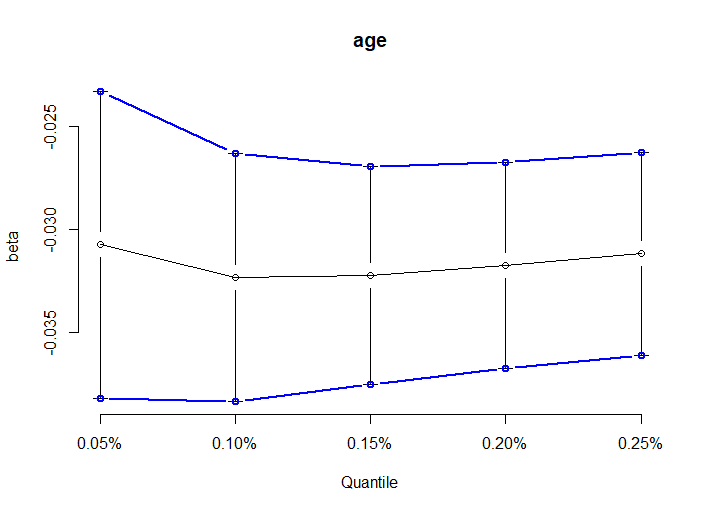
\includegraphics[width=.4\columnwidth]{age}
			\label{age}}
		\subfigure[]{
			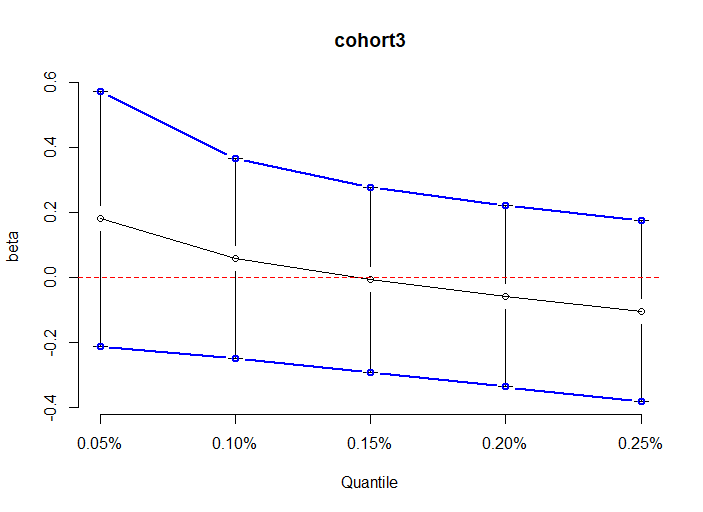
\includegraphics[width=.4\columnwidth]{cohort3}
			\label{cohort3}}
		\caption{
			$\beta$ is black line and 95\% confidence interval is blue line.
			(a) 95\% confidence interval of $\beta_{age}$ are always less than 0. 
			(b) Sign of $\beta_{cohort3}$ is changed depending on quantiles. 
			}
	\end{figure*}

%%%%%%%%%%%%%%%%%%%%%%%%%%%% Discussion %%%%%%%%%%%%%%%%%%%%%%%%%%%%

\section{Discussion}
	In this article, we proposed a regression method to estimate covariate effect in censored data given variable 

%%%%%%%%%%%%%%%%%%%%%%%%%%%% Appendix : proof of theorem and necessary lemma %%%%%%%%%%%%%%%%%%%%%%%%%%%%

\section{Appendix}

%%%%%%%%%%%%%%%%%%%%%%%%%%%% proof 1 %%%%%%%%%%%%%%%%%%%%%%%%%%%%

\subsection{Asymptotic properties of the unsmoothed estimator}
	\noindent In this part, we establish the consistency and asymptotic normality of $\beta$. We first impose the regularity conditions.
	
	\begin{enumerate}
		\item[A1] There exists $\nu \ge 0$ such that $P(C = \nu) \ge 0$ and $P(C \ge \nu) =0$.
		\item[A2] $X$ is uniformly bounded, that is $\sup_i \left\lVert X_i \right\rVert \le \infty$. 
		\item[A3] 
		\begin{flushleft}
			(i) $\beta_0(\tau)$ is Lipschitz continuous for $\tau \in [\tau_L, \tau_U]$;\\
			(ii) $f_i(t|X)$ is bounded above uniformly in $t$ and $X$,where $f_1(t|X) = dF_1(t|X)/dt$.
		\end{flushleft}
		\item[A4] For some $\rho_0 \ge 0$ and $c_0 \ge 0, inf_{b \in \beta(\rho_0)} eigmin A(b) \geq c_0$,\\ where $\beta(\rho)={b\in R^{P+1} : \inf_{\tau \in [\tau_L, \tau_U]}
			\left\lVert b-\beta_0(\tau) \right\rVert \leq \rho}$ and $A(b) = E[Z^{\otimes2}f_1 \{\exp(X^T b)|X\}]$. Here $\left\lVert \cdot \right\rVert$ is the Euclidean norm, and we define $u^{\otimes2} = uu^T$ for a vector $u$.
	\end{enumerate}
	
	\noindent \citet{peng2009competing} shows an estimator from similar estimating equation
	\begin{equation} \label{eq:9}
	S_n(\beta, \tau)=n^{-1}\sum_{i=1}^{n}X_i \Big( I\{log(Z_i-t_0) \leq X_i^{\prime} \beta\} \frac{\delta_i}{\hat{G}(Z_i)}  -\tau \Big)
	\end{equation}
	\noindent is consistent and satisfies asymptotic normality under above regularity conditions. If we change first $X_i$ to $X_i^\star$ where $X_i^\star = X_i I[Z_i>t_0]$, we are simply able to prove our suggested estimator $\beta_\tau$ is also consistent and asymptotically normal:
	\begin{math}
	n^{1/2}(\hat{\beta}-\beta_0) \xrightarrow{d} N(0, \Gamma)
	\end{math}
	\noindent where $\Gamma = A^{-1} \Sigma A^{-1}, A = \lim_{n \rightarrow \infty} X_i X_i^{\prime}f_i(0|X_i)$, and $\Sigma = \lim_{n \rightarrow \infty} Var\{U_n(\beta_0)\}$
	
%%%%%%%%%%%%%%%%%%%%%%%%%%%% proof 2 %%%%%%%%%%%%%%%%%%%%%%%%%%%%
	
	\subsection{Asymptotic properties of the smoothed estimator}
	\noindent For prove theorem \ref{thm:1}, we need following lemma \ref{lemma:1}.\\
	
	\begin{lemma} \label{lemma:1}
		Let $ W=O(n^{-1})$ any positive definite matrix, and define
		\begin{center}
			$\tilde{S}_n(\beta, \textbf{W})=\frac{1}{n} \sum_{i=1}^{n} I[Z_i \geq t_0] X_i \frac{\delta_i}{\hat{G}(Z_i)}\Phi\Big(\frac{X_i^\prime\beta-log(Z_i-t_0)}{\sqrt{X_i^{\prime} \textbf{W}X_{i}}}\Big)$
		\end{center}
		as the smoothed estimating function. Under condition 1-3, we have
		\begin{center}
			$\sup\limits_{\lVert \beta - \beta_0 \rVert \leq \epsilon_n} \lVert {n^{1/2}} \{ \tilde{S}_n(\beta, \textbf{W})-S_n(\beta) \} \rVert \xrightarrow{p} 0$, as $n\to\infty$,		
		\end{center}
		where ${\epsilon_n}$ is a positive sequence that converges to 0.
	\end{lemma}

	\noindent \textbf{Proof of lemma} \ref{lemma:1}\\
	Let $\sigma_i=(X_i^\prime W X_i)^{1/2}, \epsilon_i^\beta=X_i\beta-log(Z_i-t_0)$, and $d_i(\beta)=sgn(\epsilon_i^\beta)\Phi(-\lvert\epsilon_i^\beta/\sigma_i\rvert)$\\
	\begin{align*}
	n^{1/2}\{ \tilde{S}_n(\beta, \textbf{W})-S_n)\} & = n^{-1/2} \sum_{i=1}^{n}I[Z_i \geq t_0] X_i \frac{\delta_i}{\hat{G}(Z_i)}\bigg\{ \Phi \bigg(\frac{-\epsilon_i^\beta}{\sigma_i}\bigg)-I(\epsilon_i^\beta<0) \bigg\}\\
	& = n^{-1/2} \sum_{i=1}^{n} \frac{\delta_i}{\hat{G}(Z_i)} X_i^\star d_i(\beta)\\
	\end{align*}
	\noindent Where $X_i^\star = X_i I(Z_i>t_0)$.\\
	
	\noindent Denote $D_n(\beta)=n^{-1/2} \sum_{i=1}^{n}\frac{\delta_i}{\hat{G}(Z_i)} X_i^\star d_i(\beta)$ and $D_n^G(\beta)=n^{-1/2} \sum_{i=1}^{n} \frac{\delta_i}{G(Z_i)} X_i^\star d_i(\beta)$. It follows that
	
	\begin{equation} \label{eq:10}
	D_n(\beta)=D_n^G(\beta)-n^{-1/2} \sum_{i=1}^{n}\frac{X_i^\star\delta_i(\hat{G}(Z_i)-G(Z_i))}{\hat{G}^2(Z_i)}d_i(\beta)+o_p(1)
	\end{equation}
	
	\noindent Expectation of $D_n^G(\beta)$ is
	$E\{D_n^G(\beta)\}=n^{-1/2}\sum_{i=1}^{n}X_i^\star E{d_i(\beta)}$,
	\noindent Where 
	\begin{align*}
	E\{d_i(\beta)\} & = \int_{-\infty}^{\infty}sgn(\epsilon_i^\beta)\Phi(-\lvert\epsilon_i^\beta/\sigma_i\rvert)f_i\{\epsilon_i+X_i^{\star \prime}(\beta-\beta_0)\}d\epsilon_i^\beta\\
	& = \sigma_i \int_{-\infty}^{\infty}\Phi(-\lvert t \rvert)\{2I(t>0)-1\}f_i\{\sigma_i t + X_i^{\star \prime}(\beta-\beta_0)\}dt\\
	& = \sigma_i \int_{-\infty}^{\infty}\Phi(-\lvert t \rvert)\{2I(t>0)-1\}[f_i\{\sigma_i t + X_i^{\star \prime}(\beta-\beta_0)\}+f_i^\prime\{\omega_i^\star(t)\}\sigma_i t]dt
	\end{align*}
	\noindent Where $f_i$ is the density of $\epsilon_i=\epsilon_i^{\beta_0}$, and $\omega_i^\star(t)$ is between $x_i^{\star \prime} (\beta-\beta_0)$ and $X_i^{\star \prime} (\beta-\beta_0)+\sigma_i t$. Note that for $\beta$ that satisfies $\lVert \beta-\beta_0 \rVert \leq \epsilon_n$, where $\epsilon_n \to 0$, we have $\lVert X_i^{\star \prime} (\beta-\beta_0) \rVert \to 0$. It follows from assumption B1 that $sup_i f_i \{X_i^{\star \prime} (\beta-\beta_0)\}<\infty$ and since $\int_{-\infty}^{\infty} \Phi(-\lvert t \rvert)\{2I(t>0)-1\}dt=0$, we have $\int_{-\infty}^{\infty} \Phi(-\lvert t \rvert)\{2I(t>0)-1\}f_i \{X_i^{\star \prime} (\beta-\beta_0)\}dt=0$. In addition, by assumption B1, we can find $M>0$ such that $sup_i \lvert f_i^\prime \{\omega_i^\star (t)\}\rvert<M$. Thus, it follows that\\
	
	\begin{center}
	$\lvert E\{d_i(\beta)\} \rvert \leq \int_{-\infty}^{\infty} \lvert t \rvert \Phi(\lvert t \rvert) \lvert f_\beta, i ^\prime \{\omega_i^\star(t)\}\rvert dt \leq M \sigma_i^2 /2$
	\end{center}
	
	\noindent where the last equality holds becuase $\int_{-\infty}^{\infty} \lvert t \rvert \Phi (\{-\lvert t \rvert\})dt=1/2$.\\
	
	\noindent By assumption B2 and the fact that $W=O(n^{-1})$, $\sum_{i=1}^{n} \sigma_i^2=tr(X^\star W X^{\star \prime})=tr(W X^{\star \prime}X^\star)$ is bounded, and $\sum_{i=1}^{n} \lvert E\{d_i(\beta)\} \rvert \leq M \sum_{i=1}^{n}\sigma_i^2 /2$ is also bounded. Therefore,
	
	\begin{center}
	$\lVert E\{D_n^G(\beta)\} \rVert \leq n^{-1/2} \sqrt{p} \sup\limits_{i,j} \lvert X_{ij}^{\star} \sum_{i=1}^{n} \lvert E\{d_i(\beta)\} \rvert \to 0,\quad \text{as}\ n\to 0.$
	\end{center}
	
	\noindent In addition, by assumption B3,
	
	\begin{center}
	$Var\{D_n^{G}(\beta)\} = \frac{1}{n} \sum_{i=1}^{n} X_i^\star X_i^{\star\prime} Var \Big\{ \frac{\delta_i}{G(Z_i)} d_i(\beta) \Big\} \leq \frac{1}{n}\sum_{i=1}^{n} \frac{X_i^\star X_i^{\star\prime}}{\nu}E\{d_i^2(\beta)\}$
	\end{center}
	
	\noindent where
	\begin{align*}
	E\{d_i^2(\beta)\} & = \int_{-\infty}^{\infty}\Phi^2(-\lvert s \rvert)f_i\{\sigma_i s + X_i^\star(\beta - \beta_0)\}d(\sigma_i s)\\
	& = \int_{\lvert s \rvert > \Delta}\Phi^2(-\lvert s \rvert)f_i\{\sigma_i s + X_i^\star(\beta - \beta_0)\}d(\sigma_i s)+\int_{\lvert s \rvert \leq \Delta}\Phi^2(-\lvert s \rvert)f_i\{\sigma_i s + X_i^\star(\beta - \beta_0)\}d(\sigma_i s)\\
	& \leq \Phi^2(-\Delta)+\sigma_i \int_{\lvert s \rvert \leq \Delta}f_i\{\sigma_i s + X_i^\star(\beta - \beta_0)\}ds\\
	& = \Phi^2(-\Delta)+2\sigma_i\Delta f_i(\omega_i^\star).
	\end{align*}
	
	\noindent Note that $\omega_i^\star \in (X_i^{\star \prime}(\beta-\beta_0)-\sigma_i\Delta, X_i^{\star \prime}(\beta-\beta_0)+\sigma_i\Delta)$. Let $\Delta=n^{1/4}$ and since $\sigma_i = O(n^{-1/2})$, both $\sigma_i\Delta$ and $\omega_i^\star$ go to $0$ as $n$ increases. As $f_i(\cdot)$ is uniformly bounded around zero, both $\Phi^2(-\Delta)$ and $\sigma_i \Delta f_i(\omega_i^\star)$ go to $0$ as $n \to \infty$.\\
	
	\noindent Thus, it follows that $\lim\limits_{n \to \infty}E\{d_i^2(\beta)\}=0$, and $\lim\limits_{n \to \infty}Var\{D_n^G(\beta)\}=0$. By the Weak Law of Large Numbers, for $\beta$ that satisfies $\lVert \beta - \beta_0 \rVert \leq \epsilon_n$, we have
	
	\begin{equation} \label{eq:11}
	\lVert D_n^G(\beta) \rVert \xrightarrow{p} 0, \quad \text{as}\ n\to \infty.
	\end{equation}
	
	\noindent The second term on the right side of (\ref{eq:10}) can be written as\\
	\begin{align*}
	& n^{-1/2}\sum_{i=1}^{n} \Big\{ \frac{\delta_i X_i^\star (\hat{G}(Z_i)-G(Z_i))}{G^2(Z_i)}\Big\}d_i(\beta)+o_p(1)\\
	&= n^{-1/2}\sum_{j=1}^{n} \int_{0}^{L} \Big\{ n^{-1} \sum_{i=1}^{n} \frac{\delta_i X_i^\star d_i(\beta Z_i(u))}{G(Z_i)}\Big\} \frac{dM_j^c(u)}{y(u)}+o_p(1)
	\end{align*}
	
	\noindent where $M_i^c(u) = N_i^c(u)-\int_{0}^{t}I(Z_i\geq u)d\Lambda^c(s)$, $N_i^c(u)=(1-\delta_i)I(Z_i\leq u), \Lambda^c(u) = -log\{G(u)\}$ is the censoring cumulative hazard, $Z_i(u)=I(Z_i \geq u)$ is the ith at-risk process, and $y(u)=\lim\limits_{n \to \infty} n^{-1} \sum_{i=1}^{n} Z_i(u)$ is bounded from below in $(0,L]$ by assumption B3.\\
	
	\noindent Define $I_n(u,\beta)=n^{-1} \sum_{i=1}^{n}\frac{\delta_i X_i^\star d_i(\beta)Z_i(u)}{G(Z_i)}$, and $I(u,\beta)=E\{I_n(u,\beta)\}$. We have
	\begin{center}
		$I(u,\beta)=n^{-1} \sum_{i=1}^{n}X_i^\star E\{d_i(\beta)Z_i(u)\}$
	\end{center}
	Where $\lvert E\{d_i(\beta)Z_i(u)\} \rvert \leq E\lvert d_i(\beta) \rvert$, and
	\begin{align*}
	E\lvert d_i(\beta) \rvert & = \int_{-\infty}^{\infty} \Phi(-\lvert\epsilon_i^\beta/\sigma_i\rvert)f_i\{\epsilon_i+X_i^{\star \prime}(\beta-\beta_0)\}d\epsilon_i^\beta\\
	& = \sigma_i \int_{-\infty}^{\infty} \Phi(-\lvert t \rvert)f_i\{\sigma_i t+X_i^{\star \prime}(\beta-\beta_0)\}dt\\
	& = \sigma_i f_i\{X_i^{\star \prime}(\beta-\beta_0)\}\int_{-\infty}^{\infty} \Phi (- \lvert t \rvert)dt + \sigma_i^2 \int_{-\infty}^{\infty}t \Phi (- \lvert t \rvert) f_i^\prime \{\omega_i^\star(t) \}dt.
	\end{align*}
	
	\noindent By assumption B1, we have $f_i\{X_i^{\star \prime}(\beta-\beta_0) \}\int_{-\infty}^{\infty}\Phi(- \lvert t \rvert)dt \leq \infty$, and \mbox{$\int_{-\infty}^{\infty} t \Phi(- \lvert t \rvert)f_i^\prime\{\omega_i^{\star} \}dt\leq \infty$}. Thus, it follows that $E\lvert d_i(\beta) \rvert=)(n^{-1/2})$, and
	
	\begin{center}
		$\lVert I(u,\beta) \rVert \leq \sqrt{p} \sup\limits_{i,j} \lvert X_{ij}^{\star} \rvert n^{-1}\sum_{i=1}^{n} E \lvert d_i(\beta) \rvert = O(n^{-1/2}) \to 0$.
	\end{center}
	
	\noindent Define $\mathcal{F}=\frac{\delta_i X_i^\star d_i(\beta) Z_i(u)}{G(Z_i)}, \lVert \beta - \beta_0 \rVert \leq \epsilon_n$ and $u \in (0, \infty)$. The function class $\mathcal{F}$ is Gilvenko-Cantelli \citet{vaart1996weak} because the class of indicator functions is Gilvenko-Cantelli, and $X_i^\star, d_i(\beta), and 1/G(Z_i)$ are uniformly bounded. it follows that $sup_{\lVert \beta - \beta_0 \rVert \leq \epsilon_n, u \in (0,\infty)} \lVert I_n(u,\beta)- I(u, \beta) \rVert \xrightarrow{a.s.} 0$ and we have
	
	\begin{center}
	$n^{-1/2}\sum_{j=1}^{n} \int_{0}^{L}I_n(u,\beta)\frac{dM_j^c(u)}{y(u)}=n^{-1/2}\sum_{j=1}^{n}\int_{0}^{L}I(u,\beta)\frac{dM_j^c(u)}{y(u)}+o_p(1)$
	\end{center}
	
	\noindent By the Martingale Central Limit Theorem (\citet{fleming2011counting}), $n^{-1/2}\sum_{j=1}^{n}\int_{u}^{\beta}\frac{dM_j^c(u)}{y(u)}$ is $o_p(1)$ as n goes to infinity. It follows that, for $\beta$ that satisfies $\lVert \beta - \beta_0 \rVert \leq \epsilon_n$,
	
	\begin{equation} \label{eq:12}
	\Bigg\lVert n^{-1/2} \sum_{j=1}^{n} \int_{0}^{L} I_n(u,\beta)\frac{dM_j^c(u)}{y(u)} \Bigg\rVert \xrightarrow{p} 0
	\end{equation}
	
	\noindent Collating (\ref{eq:11}) and (\ref{eq:12}), we have
	\begin{center}
	$\lVert {n^{1/2}} \{ \tilde{S}_n(\beta, \textbf{W})-S_n(\beta) \} \rVert \xrightarrow{p} 0$.
	\end{center}
	
	\noindent for any $\beta$ such that $\lVert \beta - \beta_0 \rVert \leq \epsilon_n$. Lemma 2 is thus proven by the fact that both $\tilde{S}_n(\beta, \textbf{W})$ and $S_n(\beta)$ are monotone functions, thus the point-wise covergence could be strengthened to uniform convergence (\citet{shorack2009empirical}).\\
	
	\noindent \textbf{Proof of Theorem \ref{thm:1}}\\
	After applying induced smoothing method, $\hat{\beta}_{IS} = \beta_0+\textbf{H}^{1/2}V$ where $\textbf{H}=n^{-1}\Gamma$ and $V \sim\mathcal{N}(0,I_p)$.
	Since $\hat{\beta}_{IS}$ is a solution of
	
	\begin{equation} \label{eq:13}
	\tilde{U}_n(\hat{\beta}_{IS}, \tilde{\textbf{H}})= n^{-1} \sum_{i=1}^{n} I[Z_i \geq t_0] X_i \Bigg\{\tau -  \frac{\delta_i}{\hat{G}(Z_i)}\Phi\Bigg(\frac{X_i^\prime\hat{\beta}_{IS}-log(Z_i-t_0)}{\sqrt{X_i^{\prime} \tilde{\textbf{H}}X_{i}}}\Bigg) \Bigg\}=0
	\end{equation}
	
	\noindent Using Taylor expansion, we have
	
	\begin{equation} \label{eq:14}
	\sqrt{n}(\hat{\beta}_{IS}-\beta_0) = \frac{-\sqrt{n}\tilde{U}_n(\beta_0, \tilde{\textbf{H}})}{\tilde{U}_n^{\prime}(\beta_0,\tilde{\textbf{H}})}
	\end{equation}
	
	\noindent By Lemma (\ref{lemma:1}), $-\sqrt{n}\tilde{U}_n(\beta_0, \tilde{\textbf{H}}) \xrightarrow{p} -\sqrt{n}\tilde{U}(\beta_0)$, and \citet{kim2012censored} shows $-\sqrt{n}\tilde{U}(\beta_0) \xrightarrow{d} \mathcal{N}(0,\Sigma)$. Since $\tilde{\textbf{H}}=O(n^{-1})$, $\tilde{U}_n^{\prime}(\hat{\beta_0},\tilde{\textbf{H}})=\tilde{A}_n(\beta_0, \tilde{\textbf{H}}) \xrightarrow{p} A$. In sum,
	$\sqrt{n}(\hat{\beta}_{IS}-\beta_0) \xrightarrow{d} \mathcal{N}(0,\Gamma)$, where $\Gamma = A^{-1}\Sigma A^{-1}$.
	
%%%%%%%%%%%%%%%%%%%%%%%%%%%% references %%%%%%%%%%%%%%%%%%%%%%%%%%%%

\bibliographystyle{stco}
\bibliography{residualQR}
	
\end{document}
	
	